\documentclass[
12pt,
english,
ngerman,
headsepline,
twoside,
openright,
numbers=noenddot,version=first
]{scrreprt}

\usepackage{lmodern}
\renewcommand{\sfdefault}{lmss}
\renewcommand{\ttdefault}{lmtt}
\usepackage[T1]{fontenc}
\usepackage[utf8]{inputenc}
\usepackage{listings}
\usepackage[a4paper]{geometry}
\geometry{verbose,tmargin=3cm,bmargin=3cm,lmargin=3cm,rmargin=2.75cm,headheight=1cm,headsep=0.666cm,footskip=1cm}
\setcounter{secnumdepth}{3}
\setcounter{tocdepth}{3}
\setlength{\parskip}{\medskipamount}
\setlength{\parindent}{0pt}

\usepackage{babel}

%% include jabref file
\usepackage{caption}
\usepackage{cite}
\usepackage{courier}
\usepackage{color}
\usepackage{emptypage}
\usepackage[usenames,dvipsnames,svgnames,table]{xcolor}
\usepackage{listings}
\usepackage[printonlyused]{acronym}
\usepackage{glossaries}
\usepackage{verbatim}
\usepackage{url}
\usepackage{graphicx}
\usepackage{setspace}
\usepackage{float}
\usepackage{graphicx}
\usepackage{subcaption}
\usepackage{color}
\usepackage{csquotes}
\usepackage{totcount}
\usepackage{csvsimple}
\usepackage{amsmath}
\usepackage{rotating}
\usepackage{adjustbox}
\usepackage{tabulary}
\usepackage{lscape}
\usepackage[nomargin,inline,marginclue,draft]{fixme}
\usepackage{wrapfig}
%\usepackage{minted}
%\usepackage{fontspec}

\regtotcounter{chapter}

\setstretch{1.4}
\usepackage[unicode=true,
bookmarks=true,bookmarksnumbered=false,bookmarksopen=true,bookmarksopenlevel=2,
breaklinks=false,pdfborder={0 0 0},backref=false,colorlinks=false]
{hyperref}
\hypersetup{pdftitle={SAKWA},
pdfauthor={Dragoljub Milasinovic}}

\makeatletter

% custom colors
\definecolor{lightergray}{gray}{0.95}
\definecolor{lighterergray}{gray}{0.98}

\DeclareCaptionFont{darkgray}{\color{darkgray}}
\DeclareCaptionFont{black}{\color{black}}
\DeclareCaptionFormat{listing}{\colorbox{lightergray}{\parbox{\textwidth}{#1#2#3}}}
\captionsetup[lstlisting]{
font=sf
,format=listing
,margin=0pt
,labelfont=darkgray
,textfont=black}

\lstset{
basicstyle=\scriptsize\ttfamily,
tabsize=2,
extendedchars=true,
breaklines=true,
frame=bt,
framesep=4pt,
keywordstyle=\color{blue}\ttfamily,
%keywordstyle=\color{violet}\bfseries,
stringstyle=\color{red}\ttfamily,
%stringstyle=\color{black}\ttfamily,
commentstyle=\color{ForestGreen}\ttfamily,
%commentstyle=\color{darkgray},
rulecolor=\color{lightergray},
backgroundcolor=\color{lighterergray},
showspaces=false,
showtabs=false,
xleftmargin=17pt,
numbersep=5pt,
numberstyle=\tiny,
numbers=left,
resetmargins=true,
framexleftmargin=17pt,
framexrightmargin=6pt,
framexbottommargin=4pt,
showstringspaces=false,
morekeywords={__global__},
columns=flexible
}

\lstloadlanguages{
Java, Bash, C++
}

% create css listing style
\lstdefinelanguage{JavaScript}{
keywords={typeof, new, true, false, catch, function, return, null, catch, switch, var, if, in, while, do, else, case, break},
keywordstyle=\color{blue}\bfseries,
ndkeywords={class, export, boolean, throw, implements, import, this},
ndkeywordstyle=\color{darkgray}\bfseries,
identifierstyle=\color{black},
sensitive=false,
comment=[l]{//},
morecomment=[s]{/*}{*/},
commentstyle=\color{black}\ttfamily,
stringstyle=\color{black}\ttfamily,
morestring=[b]',
morestring=[b]"
}

% create css listing style
\lstdefinelanguage{Groovy}{
keywords={as, assert, break, case, catch ,class,const,continue,def,default,do,else,enum,extends
,false,finally,for,goto,if,implements,import,in,instanceof,interface,new,null,package,return,super
,switch,this,throw,throws,trait,true,try,while},
keywordstyle=\color{Black}\bfseries,
ndkeywords={shadowJar, class, boolean, throw, implements, import, this},
ndkeywordstyle=\color{darkgray}\bfseries,
identifierstyle=\color{black},
sensitive=false,
comment=[l]{//},
morecomment=[s]{/*}{*/},
commentstyle=\color{purple}\ttfamily,
stringstyle=\color{gray}\ttfamily,
morestring=[b]',
morestring=[b]"
}


\newcommand{\qq}{\symbol{34}} % 34 is the decimal ascii code for "
\newcommand\invisiblesection[1]{%
\refstepcounter{section}%
\addcontentsline{toc}{section}{\protect\numberline{\thesection}#1}%
\sectionmark{#1}}


%%%%%%%%%%%%%%%%%%%%%%%%%%%%%% LyX specific LaTeX commands.
\providecommand{\LyX}{L\kern-.1667em\lower.25em\hbox{Y}\kern-.125emX\@}
%% Because html converters don't know tabularnewline
\providecommand{\tabularnewline}{\\}

%%%%%%%%%%%%%%%%%%%%%%%%%%%%%% Textclass specific LaTeX commands.
\newenvironment{lyxcode}
{\par\begin{list}{}{
\setlength{\rightmargin}{\leftmargin}
\setlength{\listparindent}{0pt}% needed for AMS classes
\raggedright
\setlength{\itemsep}{0pt}
\setlength{\parsep}{0pt}
\normalfont\ttfamily}%
\item[]}
{\end{list}}

%%%%%%%%%%%%%%%%%%%%%%%%%%%%%% User specified LaTeX commands.
%% Flexibles Seitenlayout
\usepackage[automark]{scrpage2}

%% Mehrspaltenlayout ermöglichen
\usepackage{multicol}

%% Unterstützung für Farben
\usepackage{color}

%% Schönere Tabellen
\usepackage{booktabs, longtable}

%% Schönerer Blocksatz
\usepackage{microtype}


%% Mehr Platz zwischen Überschrift und Tabelle
\newcommand{\@ldtable}{}
\let\@ldtable\table
\renewcommand{\table}{ %
\setlength{\@tempdima}{\abovecaptionskip} %
\setlength{\abovecaptionskip}{\belowcaptionskip} %
\setlength{\belowcaptionskip}{\@tempdima} %
\@ldtable %
}

%% Verschiedene Symbole und Zeichen wie (c)
\usepackage{textcomp}

%% Deutsche Kurzfassung und englisches Abstract auf eine Seite
\renewenvironment{abstract}{
\@beginparpenalty\@lowpenalty
\begin{center}
\normalfont\sectfont\nobreak\abstractname
\end{center}
\@endparpenalty\@M
}{
\par
}

%% Alle Seiten vor dem Inhaltsverzeichnis sind römisch nummeriert
\pagenumbering{roman}
\let\myTOC\tableofcontents
\renewcommand\tableofcontents{
\begin{spacing}{1.1}
\myTOC
\end{spacing}
\clearpage
\pagenumbering{arabic}
}

%% Kopfzeile um Logo ergänzen
\clearscrheadfoot
\ohead{\\\headmark}
\ihead{
\includegraphics[scale=0.4]{pics/2015_10_05_THB_Logo_BW}}%\pagemark}
\ofoot[\pagemark]{\pagemark}

%% Randnotizen anpassen
%\setlength{\marginparwidth}{22mm}
%\let \oldmarginpar = \marginpar
%\renewcommand{\marginpar}[1]{%
%    \-\oldmarginpar[\raggedleft\footnotesize\sf #1]%
%        {\raggedright\footnotesize\sf #1%
%    }}

%% Zitate am Kapitelanfang
\usepackage{epigraph}
\setlength{\epigraphwidth}{9cm}

\makeatother

%-----------------------
%  Glossar https://www.sharelatex.com/learn/
%-----------------------
\makeglossaries


\begin{document}
\titlepage

\begin{center}

\includegraphics[width=12cm]{pics/2015_10_05_THB_Logo_CMYK_randlos}\vspace{0.5cm}

\par\end{center}

\vspace{1cm}

\noindent \begin{center}
\textsf{\textbf{\large BACHELORARBEIT}}\textsf{}\\

\textsf{}\\
\textsf{\huge Serverless / Serverlose Architekturen für Konventionelle Webanwendungen}
\par\end{center}{\Large \par}

\vspace{2cm}

\noindent \begin{center}
{\huge }\begin{tabular}{rl}
Vorgelegt von: & Dragoljub Milasinovic\tabularnewline
Matrikelnummer: & 20140076\tabularnewline
am: & XX. Monat XXXX\tabularnewline
\end{tabular}
\par\end{center}{\huge \par}

\vspace{1cm}

\noindent \begin{center}
zum \\
Erlangen des akademischen Grades\textsf{}\\
\par\end{center}
\noindent \begin{center}
\textsf{\textbf{\large BACHELOR OF SCIENCE}}\textsf{\textbf{\LARGE }}\\
\textsf{\textbf{(B.Sc.)}}
\par\end{center}

\vspace{1cm}

\noindent \begin{center}
\medskip{}
\begin{tabular}{rl}
Erstbetreuer: & Prof. Dr.-Ing. Schafföner\tabularnewline
Zweitbetreuer: & Jonas Brüstel, M.Sc.\tabularnewline
\end{tabular}
\par\end{center}

\noindent \begin{center}
{\huge }
\par\end{center}{\huge \par}

\newpage{}

\selectlanguage{ngerman}%
\tableofcontents{}

\pagestyle{scrheadings}


\chapter{Einleitung}{Idee-Ausführung-Markt}
\setcounter{page}{1}
\label{chap:introduction}
\epigraph{\textit{\textquotedbl{}
An idea is not a mockup\\
A mockup is not a prototype\\
A prototype is not a program\\
A program is not a product\\
A product is not a business\\
And a business is not profits.\textquotedbl{}}}{
Balaji S. Srinivasan }

Die vorantreibende Aspekte solcher Zustandsmaschine sind die Ausführung/Umsetzung der Idee bis zum Produkt und derer Beziehung zum Markt. Deren Details sind jedoch unbekannt und variabel.

Die Faktoren am Anfang einer technologischen Umsetzung einer Idee sind:
\begin{itemize}
\item Prof of Concept
\item Time-To-Market
\item Kost of Human Resources:: Skill-shortage
\item Technical technological details
\item Profitability
\end{itemize}


\section{Motivation}


Auf dem Weg zur technologischen Umsetzung einer neuen Idee liegen unbekannte Schwierigkeiten
bei der Entscheidungen über deren Umsetzung hinsichtlich auf den Architekturentwurf, die IT Infrastruktur, die Drittanbieter von Software, der Auswahl der Infrastruktur usw.
Schwierigkeiten die von spezialisierten Kompetenzen, Fertigkeiten und \glqq Know-How\grqq bedürfen.
Gehören jedoch nicht immer zum Problem des Domäns der Anwendung.

Für dieses Problem wurde \glqq FaaS\grqq als Lösung unter der Rubrik \glqq Serverless\grqq von den Hauptanbieter von \glqq Cloud\grqq Technologien vorgestellt.

Im Rahmen des Cloud-Computing handelt es sich in dieser Arbeit um eine Untersuchung der Serverless Architekturen am Beispiel einer Konventionellen Webanwendung. Dabei wird besonders geachtet ob und wie solche Technologien die Umsetzung erleichtern. Die Entwurfsmuster und die Kernfunktionalität werden mit ausschließlich Serverless Technologien am Beispiel von KOMA mit AWS umgesetzt.


\section{Ziel}
\label{sec:task}
\newacronym{MVP}{Mivip}{Minimal Viable Product}
@acronym MVP Minimal Viable Product : \cite{rady2016serverless} Das Ziel ist ein MVP Minimal Viable Product in form eine @acronym SPA Single Page Application mit ausschließlich \glqq Serverlosen\grqq Architekturen vor zur Verfügung zu stellen.

Nach der Umsetzung werden die Erfahrungen und Ergebnisse ausgewertet, um dem Leser bei dem Entscheidungsprozess bei der Umsetzung einer Webanwendung besser zu Informieren.

Die Webanwendung soll möglichst für zukünftige Änderungen flexibel sein.

\section{Aufbau der Arbeit}
\label{sec:layout}

Zuerst wird den Leser in die Serverless \ref{sec:serverless} Technologien eingeführt, das Programmiermodell vorgestellt
und die Entscheidungsprinzipien\ref{par:serverless-principles} erläutert.
Als Zweites wird KOMA \ref{sec:KOMA} als vorläufiges Beispielanwendung und deren Anforderungen vorgestellt.
Nach dem Überblick, lässt sich die Umsetzung besser \glqq Bottom-Up\grqq verstehen.
Am Ende wird es darüber diskutiert, welche TradeOffs entstehen und die Zukünftperspektiven von Serveless Technologien/ Architekturen.

\chapter{Grundlagen}
\label{chap:principles}
\epigraph{\textit{\textquotedbl{}
There are only two hard things in computer science:\\ cache invalidation and naming things.\textquotedbl{}}}{ Phil Karlton }

Service Orientierte Architektur SOA unterlegt die Annahme dass, ein System aus mehreren kleinen, austauschbaren und entkoppelten Diensten bestehen kann. Microservices und Serverless versuchen die Komplexität der SOA anzusprechen. Beide Ansätze zwingen auf Separation of Concerns, häufige Deployments und Heterogeneous DSL Domain Specific Language selection.
Auf einer Seite Microservices können ihren Zustand und Daten halten und werden mithilfe von \glqq Frameworks\grqq implementiert. Auf der anderen Seite Serverless sind Zustandlos.
ConnectWise\footnote{ConnectWise: \url{https://aws.amazon.com/solutions/case-studies/connectwise/}}, Netflix\footnote{Netflix: \url{https://aws.amazon.com/solutions/case-studies/netflix-and-aws-lambda/}} und UNLESS\footnote{UNLESS: \url{https://unless.com/}} sind beispiele von Unternehmen die von Serverless Architekturen profitieren.

\section{Architekturen}

Die Architekturentwurfsmuster helfen uns zu kommunizieren welches Zweck unsere Software erreichen möchte und bieten generische Lösungen für wiederkehrende Probleme bei der Softwareentwicklung.

Separation of concerns
Reusable layers
Maintenance @Schafföner JEE1
Koma standalone snapshot
Components:
Controller: router, handle in-req build out-res
Service: @Transaction
Repository: 1-1 mapping to db

Wenn eine erfolgreiche Codeänderung von andere Änderung abhängt, soll die Architektur überprüft werden.


Für Konventionelle Webanwendung wird hier damit gehalten, als ein System das über Presentation, Data, and Application/Logik Tiers/Stufe verfügt. Jede Stufe kann mehreren Logik-Layers/Lagen enthalten, die für unterschiedlichen Funktionalitäten des Domäns verantwortlich sind. Logging wäre ein beispiel für Cross-Cutting Concern der Layers hinaus ausspannt. Die Komplexität wächst mit der Beschichtung zusammen.\\
Tier = Major Component System eg. Presentation Data
Layer = Logical Responsability or Funtionality Domain

Serverless versucht das System in Funktionen runter zu brechen und auf ihnen das sichere Zugang dem Front-End zu erlauben.

\section{Serverless}
\label{sec:serverless}

Serverless ist ein @Glossar Web Dienst/Service von Cloud-Anbieter, wird auch als @Glossar FaaS bezeichnet. Welcher grundlegende Serverinfrastruktur vom Cloud-Anbieter wie Amazon Web Services verwaltet wird. Komplexe Probleme wie horizontale und vertikale Skalierbarkeit, Fehlertoleranz, Flexibilität werden von Kunden und Benutzer nur noch nach bedarf Konfiguriert.


Prinzipien\label{par:serverless-principles} von Serverless Architeturen: \cite{sbarski2017serverless}
Rechen-Dienst dass, nach Anfrage isoliert, unabhängig und granular ausgeführt wird.
SRP Single Responsability Prinzip: Funktionen werden dadurch mehr Testable/Prüfbar. Deren Vernetzung erlaubt komplexe Systeme zu entwerfen, die dank der Stateless Natur der Funktionen schnell zu skalieren sind.
Diese Vernetzung kann durch einen Push-Based Event driven Pipe-line.
Um die Komplexität des Systems zu reduzieren und die längerfristige Wartbarkeit zu verbessern, wird der Controller und/oder Router im Client und Third Party Dienste hinzugefügt.

In einem beispielhaften konventionellen AdServer, nach einem Click auf eine Werbung wird eine Nachricht über ein Kanal an einen Clickprozessor, derer Laufzeit eine Anwendung ist, geschickt. Im Serverless wird dieser Clickprozessor als Funktion pro Nachricht instantiiert derer Laufzeitumgebung und Messagebroker der Cloudanbieter liefert.

\subsection{Use Cases}

\subsection{Architecturen}

\subsection{Muster}

Befehlmuster wird bei Fusekiserver\ref{komponenten:fuseki} als erteiler der Httpanfrage indem die SparQL Abfrage weiterleiten kann. Daher wird ein Pfad haus/hunde und haus/katze zur gleichen Funktion führen.
Dieser kann aber offline gehen, also mehreren priorisierten MessagePattern als Queue vor eine oder mehreren Lambdas zu setzen absichert die Stabilität des Systems und entkoppelt Komponenten @RoundRobin?? BSRN.
Die Verkettung von Funktionen mittels \glqq Pipes\grqq erlaubt die mehrfache Filterung von Daten.

%Stand der Technik: 
%Vorgehensweise bei Traditionelle Webanwendungen:  
%Software Architektur: "What's important". Frühe, un-/schwer- veränderbare Entscheidungen.
%@Glossar: 
%Web Services are processes that expose their interfaces to the Web so that users can invoke them. %Facilitate service discovery and meaning encoded in schemas


%Design: Lambda Orchestrator -> Pool of Lambdas to use

\section{KOMA}{Beispiel Anwendung}
\label{sec:KOMA}

Die heutige Rahmenlehrpläne sind nicht mehr fachlich sondern nach Kompetenzentwicklung orientiert, um Kompetenzprofile für Lerner zu gestallten. @cite aber wenn?
Das Modell von KOMA basiert auf dem Grundmodell von
@ref \glqq European Qualifications Framework Semantics\grqq und dem deutschen Qualifikationsrahmen. <-- really?

\glqq KOMA\grqq ist ein Akronym für Kompetenz-Matrix. Die Umsetzung der Anwendung soll die von einem Individuum oder Schüler
erworbene und zu erwerbenden Kompetenzen und deren Niveau nachvollziehen.
Der Kompetenzstand einer Person ist mit dem EQF-Rahmen @Acro vergleichbar, und daher International anerkennbar.

%Diese soll für die pädagogische Diagnostik und Intervention genutzt werden.
Wenn diese Anwendung in Bildungsintitutionen eingesetzt wird, dienen die Rahmenlehrpläne als Leitpfad für die Belegung der einzelnen Kompetenzen
und KOMA für die Organisation der einzelnen Fachrichtungen. Der Kern solcher Org. ist die Zuweisung von Aktivitäten auf vordefinierten Kompetenzen.
Aktivitäten lassen sich einzeln oder in einer Sequenz anordnen. Sequenzen werden in LVen zusammengestellt. So können Aktivitäten, Sequenzen und Kompetenzen
als gestalltungsmittel für LV benutzt. Das Modell verfügt von eine Figur um die erledigte Aktivitäten auszuwerten, nämlich Evaluation.

Wegen der Kompetenzorientierung, wird Kompetenz als Unit-Of-Work betrachtet für Modelierungszwecke.

\paragraph{Hochschule Beispiel}
Beispiel:
Der Lehrplan fordert die Kompetenzen K in K1, K2, K3 .. Kn für den Bachelordiplom. Nach deren Manuellen Eingabe werden automatisch
ihren Requirenments/Anforderungen/Abhängigkeiten Baum erzeugt. Dadurch können bereiche des Baums als LV betrachtet werden und Kompetenzen aufeinander
bauend für eine Klassenstufe/Semestergang sequenziert werden. Die Auswertung der Ergebnisse der Aktivitäten und die Aktualisierung des Kompetenzstands
des Schulers folgen.

\paragraph{Schule Beispiel}
Allgemeines Beispiel:

Beispielsweise drückt sich die Kompetenz beim Erwerb einer Fremdsprache – wenn mankommunikative Handlungsfähigkeit als Bildungsziel vorgibt – darin aus, wie gut man kommu-nikative Situationen bewältigt, wie gut man Texteunterschiedlicher Art verstehen und selbst adressatengerecht Texte verfassen kann, aberunter anderem auch in der Fähigkeit, gram-matische Strukturen korrekt aufzubauen und bei Bedarf zu korrigieren, oder in der Fähigkeitund Bereitschaft, sich offen und akzeptierend mit anderen Kulturenauseinander zu setzen. Standards für das Fremdsprachenlernen müssen diese Teilkompetenzen darstellen und je-weils verschiedene Niveaustufenunterscheiden (vgl. Anlage a). Hierbei spielen nicht nurkognitive Wissensinhalte eineRolle;diese sind vielmehr– wie Weinert im obigen Zitat her-vorhebt und das zuletzt genannte Beispiel der sog. Interkulturellen Kompetenz besonders deutlich macht – mit Einstellungen, Werten und Motiven verknüpft.
Kompetenzen spiegeln diegrundlegenden Handlungsanforderungen, denenSchülerinnen und Schüler in der Domäneausgesetzt sind. Durch vielfältige, flexible und variable Nutzung und zunehmende Vernetzungvon konkreten, bereichsbezogenen Kompetenzen können sich auch „Schlüsselkompetenzen“entwickeln, aber der Erwerb von Kompetenzen muss – wie Weinert (2001) hervorhebt – beim systematischen Aufbau von „intelligentem Wissen“ in einer Domäne beginnen.
- Jede Kompetenzstufe ist durch kognitive Prozesse und Handlungen von bestimmter Qualität spezifiziert, die Schüler auf dieser Stufe bewältigen können, nicht aber Schüler auf niedrigeren Stufen. Zum Bildungsstandard gehört, dass für einzelne Jahrgänge festgelegt wird, welche Stufen die Schülerinnen und Schüler erreichen sollen.

\paragraph{Use Case}
Ein Nutzungs-Fall aka. Use-Case:
-Als Professor, will ich eine Auflistung der erworbene Fertigkeiten einer Klassenstufe abrufen können.

-Als Professor, will ich das Kompetenzniveau einer Kompetenz eines Studenten und deren Fertigkeiten abrufen können.

-Als Student, will ich mein Kompetenzprofil für meinen Lebenslauf benutzen.

\chapter{Umsetzung}
Die grundlegende Vorgehensweise bei der Umsetzung dieses Projekts wird Analyse, Entwurf, Implementierung und Test sein. Der Forschender Charakter dieses Projekts lässt sich nicht Testgetrieben implementieren.
Das



\section{Komponenten}

Um dem Leser einen Anhaltspunkt zu verleihen, werden hier die Softwarekomponenten beschrieben.

\begin{figure}[H]
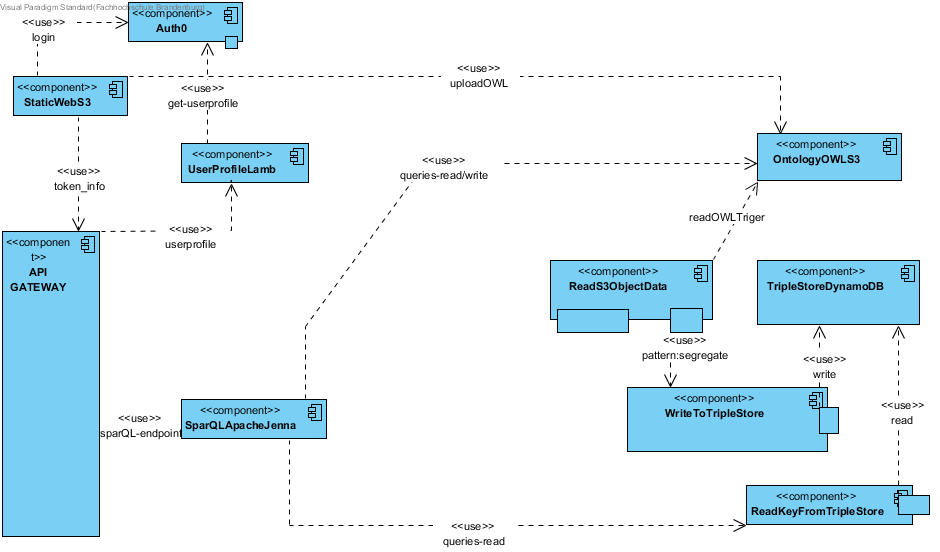
\includegraphics[width=\linewidth]{pics/arch-comp.png}
\end{figure}

legacy api proxy\cite{sbarski2017serverless}
lambda<convert/invoke> fuseki-server\label{komponenten:fuseki}

nice: graphQL= json matcher over multiple DBs


\section{Anforderungen Analyse}

Zu den Anforderungen
\begin{itemize}
\item Mit dem EQF vergleichbare Kompetenzeindefinitionen
\item Von Browser abrufbar
\item Private Datenspeicherung u.d Login
\item Zukünftige Erweiterungen berücksichtigen
\item Ertrag von großen Nutzlastschwankungen
\end{itemize}


\section{Datenhaltung Analyse und Auswahl}

Die Polymorphe Gestaltung von Kompetenzmodellen und deren zukünftige Weiterentwicklung stellt die Benutzung des traditionellen RDBMS für KOMA in Frage. Im Folgendem werden die Eigenschaften von relationalen mit ontologischen Schemas verglichen.


%@Pre-Dev--> Tabelle 
\begin{table}
\caption{Vergleich relationalem mit ontologischem \ref{subsec:ontology} Schema}

\centering{}
\begin{tabular}{ccc}
\noalign{\vskip\doublerulesep}
Eigenschaft & Relational & Ontologisch \tabularnewline[\doublerulesep]
\hline\noalign{\vskip\doublerulesep}
Darstellung Welt-Annahme & Existiert nur & Existiert mindestens \tabularnewline[\doublerulesep]
\noalign{\vskip\doublerulesep}
Individual & muss Unique & kann >= 1 \tabularnewline[\doublerulesep]
\noalign{\vskip\doublerulesep}
Info & Ableitung = x & ja \tabularnewline[\doublerulesep]
\noalign{\vskip\doublerulesep}
Oritentation & Data & Bedeutung \tabularnewline[\doublerulesep]

\end{tabular}
\end{table}

%@Pre-Dev::Feasibility Study
Es wurden folgende Faktoren für die Entwicklung einer Ontologie erkannt:
%@list
\begin{itemize}
	\item Zirkuläre Abhängigkeiten sind zugelassen
	\item Equivalenzklassen zwischen KOMA und andere Ontologie soll die Anerkennung von erworbenen Kompetenzen ermöglichen
	\item Die Begriffe der Kompetenzen können sich ändern oder die Ontologie soll erweitert werden
	\item Die Verbindung zu externen Ontologien kann neues Wissen ableiten
\end{itemize}

6.2.2 \cite{OntoCloud}Benefits on Interoperability and Linked-Data by Using
Ontology Engineering

Es handelt sich daher um eine \glqq Linked Data Driven Web Application\grqq.%@href 
Dieser Begriff gehört zum \glqq Semantic Web\grqq,der in der Sektion der Ontologie\ref{subsec:ontology} weiter erläutert wird.

\section{Semantic Web}

Das \glqq Semantic Web\grqq ist eine Erweiterung des herkömmlichen Web, in der Informationen mit eindeutigen Bedeutungen versehen werden\cite{OntoWhat2}.
set of standards and best practices for sharing data and the semantics of that data over the Web for use by applications\cite{SparqlLearn} .
 Diese Bedeutungen werden für Maschinen durch Ontologien dargestellt. 
Die Ontologien werden in der OWL2 Spezifikation von W3C\footnote{WWW Consortium \url{https://www.w3.org/standards/semanticweb/}}beschrieben. Die hälfte der Linked Datenbasis sind veroffentlicht. 

\begin{figure}[h]
	\centering
	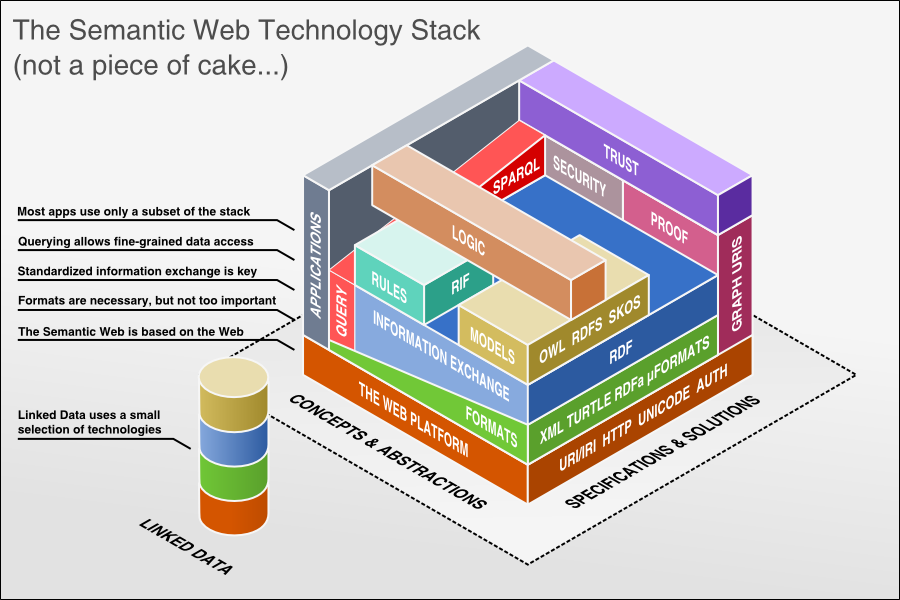
\includegraphics[width=0.8\textwidth]{pics/semantic_web_technology_stack.png}
	\caption{Überblick von benutzten Technologien}
	\label{fig:semantic-web-stack}
\end{figure}

\section{Ontologie}{Konzeptuelle Modellierung}
\label{subsec:ontology}

%@Def
Eine Ontologie ist eine formale Spezifikation über eine Konzeptualisierung\cite{OntoWhat}. Die Denotation jeweiliger dargestellten Signifikanten lässt sich durch seinen weltweit eindeutigen Präfix identifizieren. Deren Beziehungen können auch zu externen Ontologie-signifikanten verweisen und dadurch ein Consensus über Begrifflichkeiten. 

Während der Umsetzung wurde Protege\footnote{\url{http://protege.stanford.edu}: "This work was conducted using the Protégé resource, which is supported by grant GM10331601 from the National Institute of General Medical Sciences of the United States National Institutes of Health."} benutzt.
Der Entwurf der Ontologie wurde nach Ontology-Engineering-101 durchgeführt:

Die auf die Entwicklung vorbereitende Aufgaben folgen.

\paragraph{Software Plattform} Zunächst es wird die Plattform der zu entwickelnde Software der Anwendung festgelegt.
%@Pre-Dev::Environ
%Software platform ? 
Die Daten können in Produktion mittels einer \glqq Triple-Store\grqq mit grundsätzlich 4 alternativen gespeichert:
\begin{itemize}
	\item Monolitische Triple Speicherung
	\item Property Werte
	\item Vertikal Partitionierte Tables
	\item Hexastore
\end{itemize}

Die für KOMA unterstützende Infrastruktur wird ein Rechner mit Browser wie Firefox oder Chrome und die AWS Dienste wie Lambda, API Gateway und S3. Das Kommunikationsprotokoll auf der Anwendungsebene zwischen Endpunkten ist HTTP v1.1.
Eine Ontologie kann mittels Sparql abgefragt werden. Sparql ist eine Abrfragesprache für RDF, Spreadsheets, XML und JSON formate\cite{SparqlLearn}. Wir beschreiben die Ontologie mit dem Datenmodel RDF und der TURTLE syntax.

Für die Entwicklung und als MVP eignet sich S3 @Acro für die Speicherung von großen Datenmengen. Der nächste Schritt wird eine Indexierung der URIs jeweiliger Subject, Predicate und Object in DynamoDB. 

Die Ausführung von Abfragen auf die Ontologie wird direkt mithilfe von \glqq Jena SPARQL ARQ\grqq Framework realisiert. Deren Quelldateien werden in einer Lambda @Acro Funktion ausgeführt.

\paragraph{Der Umfang der Ontologie} ist die Konkrete Fragestellungen für die pädagogische Diagnostik und Intervention von Fortschritten der Studierenden im Kompetenzrahmen der Lehrpläne.

\begin{itemize}
	\item Welche stand von Kompetenzen hat eine Klassenstufe?
	\item Welche Kompetenzrückstände oder Auffälligkeit sind von eine Klassenstufe erkennbar?
	\item gegeben sei ein Kompetenzstand, welche Leistung kann ich von eine Klassenstufe erwarten?
\end{itemize}


Um die Neuerfindung des Rades zu vermeiden, die Recherche ergab einen aktuell öffentlichen graphischen ontologischen Entwurf\cite{OntoMoodle} siehe\ref{fig:competence-ontology} der in Moodle mit eine Relationalen Datenbasis und PHP umgesetzt. Nach dessen Ontologien wurde mittels Watson\footnote{Watson \url{http://watson.kmi.open.ac.uk/WatsonWUI/}} und LOD\footnote{LOD Cloud \url{http://lod-cloud.net/}} nichts öffentlich gefunden. 

\begin{figure}[h]
	\centering
	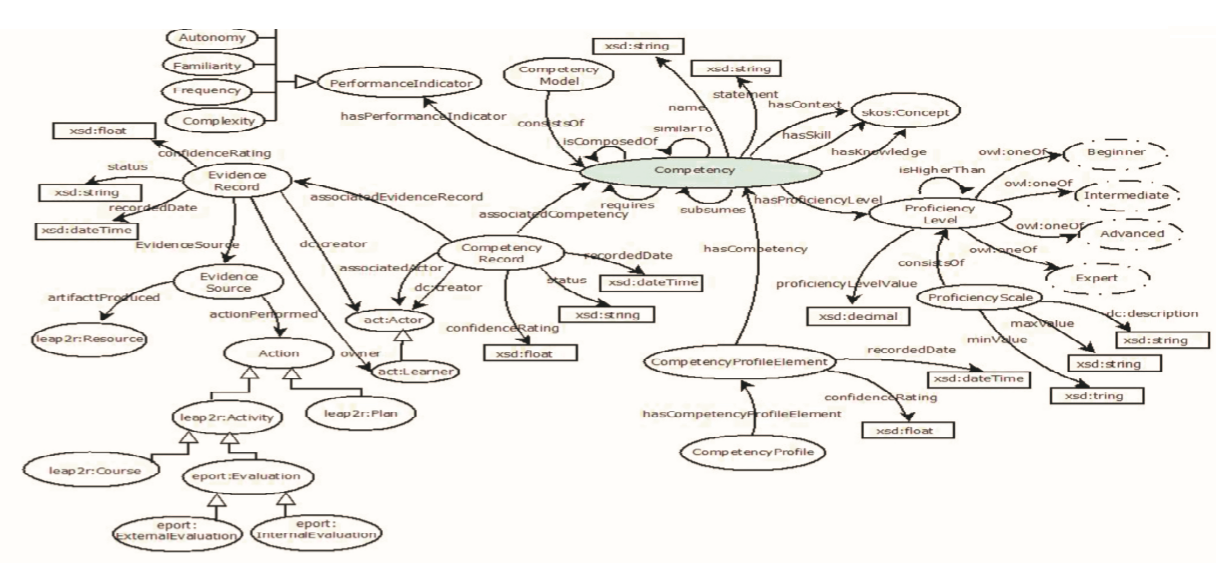
\includegraphics[width=\linewidth]{pics/competency-ontology.png}
\caption{Kompetenzontologie}
\label{fig:competence-ontology}
\end{figure}

Bei der Analyse lässt der Entwurf und dessen Dokumentation freie Interpretation über Begriffe und deren Zweck, beispiele davon sind \glqq isComposedOf\grqq, \glqq subsumes\grqq. Ein Standard zur graphischen Darstellung ist zur Zeit?? noch nicht anerkannt.@Cite research-gate graphol

Anderseits wurde ein \glqq EQF Framework\footnote{EQF Beschreibung \url{https://ec.europa.eu/ploteus/content/descriptors-page}}\grqq für Ontologien beschrieben, aber nicht öffentlich umgesetzt. Es bietet dabei eine europäisch anerkannte Definition von Kompetenz, nämlich RCD\cite{EQFCompetency}


\begin{wrapfigure}{i}{0.36\textwidth}
	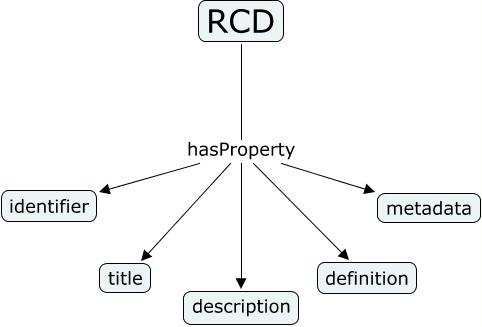
\includegraphics[width=0.9\linewidth]{pics/RCD.jpg}
\end{wrapfigure}


Daher folgt eine beispielhafte Auflistung der auf unseren Anwendungsfall angepasste und ergänzende Interpretation der dargestellten Terminologie des Entwurfs und der RCD.


\paragraph{Auflistung der Terminologie}\ref{tab:terms} Die zwei Leitmotive sind auf eine Seite \underline{Kompetenzanforderungen}: sie legen fest, über welche Kompetenzen ein Schüler, eine Schülerin verfügen muss, wenn wichtige Ziele der Schule als erreicht gelten sollen. Systematisch geordnet werden diese Anforderungengen in Kompetenzmodellen, die Aspekte, Abstufungen und Entwicklungsverläufe von Kompetenzen darstellen\cite{Competence}. Und auf der Anderen nach \underline{\Gls{Kompetenz}} als die bei Individuen verfügbaren oder durch sie erlernbaren kognitiven Fähigkeiten und Fertigkeiten, um bestimmte Probleme zu lösen, sowie die damit verbundenen motivationalen, volitionalen und sozialen Bereitschaften und Fähigkeiten, um die Problemlösungen in variablen Situationen erfolgreich und verantwortungsvoll nutzen zu können\cite{weinert2002leistungsmessungen}.


\newglossaryentry{Kompetenz}{name={Kompetenz},description={die bei Individuen verfügbaren oder durch sie erlernbaren kognitiven Fähigkeiten und Fertigkeiten, um bestimmte Probleme zu lösen, sowie die damit verbundenen motivationalen, volitionalen und sozialen Bereitschaften und Fähigkeiten, um die Problemlösungen in variablen Situationen erfolgreich und verantwortungsvoll nutzen zu können}}




\begin{table}[H]
\caption{Terminologie}\label{tab:terms}


\noindent \centering{}\begin{tabular}{ccc}
\hline
\noalign{\vskip\doublerulesep}
Darstellung & Begriff & Bedeutung\tabularnewline[\doublerulesep]
\hline
\noalign{\vskip\doublerulesep}
Competence & Kompetenz & Kontext adäquate Anwendung von Fertigkeiten \tabularnewline[\doublerulesep]
\noalign{\vskip\doublerulesep}
CompetenceProfile & Kompetenzprofil & Sammlung von Kompetenzen \tabularnewline[\doublerulesep]
\noalign{\vskip\doublerulesep}
Competence & Kompetenz & Kontext adäquate Anwendung von Fertigkeiten \tabularnewline[\doublerulesep]
\noalign{\vskip\doublerulesep}
Skill & Fertigkeit & Das systematisch Tun-Können einer Aufgabe \tabularnewline[\doublerulesep]
\noalign{\vskip\doublerulesep}
Knowledge & Wissen & Verstehen von Informationen
\tabularnewline[\doublerulesep]
\noalign{\vskip\doublerulesep}
Other & Andere & Nicht kategorisiert aber zu beachten
\tabularnewline[\doublerulesep]
\noalign{\vskip\doublerulesep}
ProficiencyLevel & Kompetenzniveau & Bewertung einer Kompetenz
\tabularnewline[\doublerulesep]
\noalign{\vskip\doublerulesep}
PerformanceIndicator & Kompetenzmaß & Kriteria zur Auswertung
\tabularnewline[\doublerulesep]
\noalign{\vskip\doublerulesep}
Course|LV & Lehrveranstaltung & Sammlung von Sequenzen
\tabularnewline[\doublerulesep]
\noalign{\vskip\doublerulesep}
Sequenz & Sequenz & Sammlung von Aktivitäten
\tabularnewline[\doublerulesep]
\noalign{\vskip\doublerulesep}
Activity & Aktivität & Lernaktivität
\tabularnewline[\doublerulesep]
\noalign{\vskip\doublerulesep}
Action & Aktion & Lerntat
\tabularnewline[\doublerulesep]
\noalign{\vskip\doublerulesep}
Actor & Täter & Aktiver Agent aka Lerner
\tabularnewline[\doublerulesep]
\noalign{\vskip\doublerulesep}
Learner & Lerner & Kompetenz erwerbender Agent
\tabularnewline[\doublerulesep]
\noalign{\vskip\doublerulesep}
CompetencyRecord & Kompetenzaufnahme & --
\tabularnewline[\doublerulesep]
\noalign{\vskip\doublerulesep}
EvidenceRecord & Kompetenzbeweis & --
\tabularnewline[\doublerulesep]
\noalign{\vskip\doublerulesep}
EvidenceSource & Kompetenzherkunft & --
\tabularnewline[\doublerulesep]
\noalign{\vskip\doublerulesep}
todo & todo & todo
\tabularnewline[\doublerulesep]
\noalign{\vskip\doublerulesep}
todo & todo & todo
\tabularnewline[\doublerulesep]
\hline
\end{tabular}
\end{table}

\paragraph{Klassenhierarchie}
Um Wissen abzuleiten und Inkonsistenzen zu identifizieren werden die Klassen und Properties durch Restrictions versehen oder definiert. Folgende Restrictions wurden angewendet.
\begin{table}[H]
\caption{Klassendefinition}

\noindent \centering{}\begin{tabular}{cc}
\hline
\noalign{\vskip\doublerulesep}
Klasse & Definition \tabularnewline[\doublerulesep]
\noalign{\vskip\doublerulesep}
LV & $only Sequenz$ \tabularnewline[\doublerulesep]
\end{tabular}
\end{table}

@Build : ableitungs Baum von Protege an stelle von Tabelle

\paragraph{Properties und Attributen von Klassen}

\begin{table}[H]
\caption{Properties}\label{tab:prop}

\noindent \centering{}\begin{tabular}{cc}
\hline
\noalign{\vskip\doublerulesep}
isComposedOf & $\forall{Class} \equiv only Class$ \tabularnewline[\doublerulesep]
\noalign{\vskip\doublerulesep}
subsumes & $\exists{Class} \equiv some Class$ \tabularnewline[\doublerulesep]
\end{tabular}
\end{table}


\section{RDF}

Die bisher erreichte Analyse des Domänsproblems soll nun anhand Protégé in einen RDF format beschrieben werden. Der Menschen lesbarsten RDF Format ist TURTLE. Seine Syntax besteht aus Triples mit \glqq .\grqq beendete Zeilen. Ein Triple stellt ein Fakt dar, un besteht aus einem Subjekt, einem Prätikat und einem Objekt. Diese können sich in TURTLE verschachteln wie das folgende Listing\ref{lst:turtle} zeigt.

\begin{lstlisting}[language=SQL,caption={Darstellung von Triples in TURTLE},label={lst:turtle}]
:EvidenceRecord rdf:type owl:Class .

:actionPerformed rdf:type owl:ObjectProperty ;
rdfs:domain :EvidenceSource ;
rdfs:range :Action .
\end{lstlisting}


\section{Sparql}

Um aus Ontologien Informationen zu entnehmen, wird die Abfragesprache \glqq SPARQL\grqq @Acro verwendet. 
Diese ist ähnlich zu SQL. Mit dem Programm \glqq Protétegé\grqq können SPARQL Abfragen lokal ausgeführt werden.

\begin{lstlisting}[language=Sparql]
SELECT * WHERE { ?s ?p ?o .}
...
\end{lstlisting}

Nach der Modellierung in Protégé wird die OWL Datei in einem S3 Bucket verpackt und dadurch deren Zugriffsrechte konfiguriert, so dass in Produktion nur eine berechtigte Anfrage z.B. von eine Lambda Funktion oder DynamoDB angenommen wird. 

\begin{lstlisting}
{
"Version": "2012-10-17",
	"Statement": [
		{
			"Effect": "Allow",
			"Action": "s3:*",
			"Resource": "*"
		}
				]
}
\end{lstlisting}

So dass auch die Benutzer von KOMA solche Abfragen stellen können wird ein \glqq Sparql-endpoint\grqq mit Hilfe von Apache Jena ARQ, ein Sparql-Engine, zur Verfügung gestellt. 
%Fuseki ist ein Server zur Verwaltung von Sparqlabfragen und deren Transaktionen. @Cite CRUD und ACID RDB in sparql.
%Fuseki wird Embedded benutzt.
Dieser Sparql-Endpoint entspricht der Repositoryschicht der Anwendung und wird nach Anfrage von der Ontologie in S3 mittels Sparql JSON Objekte zurückliefern.
Eine Lambdafunktion arbeitet als Schnittstelle \ref{lst:lambda-interface} zwischen die ARQ Bibliothek, den Client und die darunterliegende Infrastruktur.

\begin{lstlisting}[language=Java,caption={Schnittstele Lambda},label={lst:lambda-interface}]
public class Handler implements RequestHandler<RequestClass, String> {

@Override
public String handleRequest(RequestClass input, Context context) {
	return new Controller(System.getenv(ENV_BUCKET)
						  , Regions.US_WEST_2.getName())
								.executeQuery(request.getQuery()
								, request.getBucketKey());
	}

}

\end{lstlisting}

Um sich von die durch Lambda entstandene Abhängigkeit möglichst entkoppelt\cite{FlowerRefactoring} zu halten, wird das Modul von Jena-ARQ nur als externe Abhängigkeit des Lambdaprojektes zugewisen.
Die AWS Lambda stellt eine Interface zur Verfügung und der Nutzer die zu benutzende Bibliotheken zusammen in eine JAR Datei verpackt. Dem entsprechend wird der Buildscript von Gradle\cite{Muschko2014} angepasst\ref{lst:gradle}. 

\begin{lstlisting}[language=Groovy,caption={Abhängigkeitenverwaltung für Lambda in Java},label={lst:gradle}]
plugins {
	id 'com.github.johnrengelman.shadow' version '2.0.1'
	id 'java'
}
shadowJar {
	mergeServiceFiles()
}
...
$ gradle clean build shadowJar
\end{lstlisting}

Die AWS Console lässt die Funktionen hochladen und konfigurieren, ohne nötige Kenntnisse von der AWS-CLI. Zusätzlich muss der RESTful Pfad auf die verantwortliche Funktion in API Gateway zugewiesen werden. 


Um den Datenmodell möglichst simpel programmatisch abzufragen wird zunächst dessen Schnittstelle\ref{sec:rest} definiert. 

\section{RESTful API}
\label{sec:rest}

Die Komplexität des darunterliegenden Datenmodells erlaubt eine RESTful\cite{Hunter2017} Schnittstelle nur einfache abfragen zu formulieren. Daher zusätzlich ein Endpunkt\ref{tab:rest} für Komplexe Sparql Abfragen, die im Body des HTTP Requests in JSON geschickt wird. 

\begin{table}[H]
	\caption{RESTful API}\label{tab:rest}
	\noindent 
	\centering{}
	\begin{tabular}{ccc}
		\hline
		\noalign{\vskip\doublerulesep}
		Methode & URL & Rückgabe\tabularnewline[\doublerulesep]
		\hline
		\noalign{\vskip\doublerulesep}
		GET & /ontology & Information über KOMA
		\tabularnewline[\doublerulesep]\noalign{\vskip\doublerulesep}
		\noalign{\vskip\doublerulesep}
		GET & /ontology/\{individual\} & RDF von Individual
		\tabularnewline[\doublerulesep]\noalign{\vskip\doublerulesep}
		GET & /page & Auflistung von Entitäten 
		\tabularnewline[\doublerulesep]\noalign{\vskip\doublerulesep}
		GET & /page/\{individual\} & Information über diesen Fakt
		\tabularnewline[\doublerulesep]\noalign{\vskip\doublerulesep}
		POST & /sparql & Abfragenergebnis
		
	\end{tabular}
\end{table}

AWS API Gateway ermöglicht die Definition, Konfiguration und das Importieren von Schnittstellen. Beispielsweise kann die Abfrage GET https://<host>/page/\{individual\} 

\begin{lstlisting}[language=Javascript,caption={Mapping Template},label={lst:map-template}]
GET https://<host>/page/{individual} 
...
{
"individual" : "$input.params('individual')"
}
\end{lstlisting}

Damit wurde die zu erwartende Eingabe für den Sparql-Endpoint definiert. Der Zugang auf die Schnittstelle wird durch CORS konfiguriert um deren Ausnutzung zu vermeiden. 

Dieser Endpunkt unterstützt nicht nur GET-Abrufe, sondern auch POST-Anforderungen mit einer Nutzlast.
Unter der verfügbaren SparQL endpoints Implementierungen




\section{DevOps}
<-- hier wegen JSON konfigurationene in AWS und un endliche fefehle in AWS cli erzählen ?? 
excurs zu Serverless Frameworks 

\section{Single Page Application}

Da KOMA ohne Vorkenntnisse gebrauchsfertig sein soll, mit dem Fakt dass Milliarden von Desktop Geräte die Web mit einem Browser erkundigen können, lässt sich die Entscheidung über die Art der Benutzeroberfläche leicht Treffen.

Die Web Anwendung ist für alle Rechenaufgaben verantwortlich die im Browser aus dem Sicherheitssichtpunkt kein Gefahr darstellen, um den Backend oder Servers möglichst wenig auszulasten. Deswegen bietet sich eine Single Page Application an. 
Die SPA besteht aus ein einziges HTML Dokument. Dies vereinfacht man die Konfiguration der Authentifizierung und unterbricht den Fluss der UI-Darstellung zwischen Seiten.

Ein konfiguriertes Anfangsprojekt/Quickstart kann mithilfe von Initializr\footnote{Initializr \url{http://www.initializr.com/}} oder JHipster\footnote{JHipster \url{http://www.jhipster.tech/}}. Für die lokale Entwicklung der Webseite werden anhand von NodeJS und NPM folgende Bibliotheken als Abhängigkeiten verwaltet: Bootstrap als Stylescheet und jQuery als Javascript-Bibliothek.
Die Webseite wird Statisch mittels S3 geliefert. Dies geschieht mit einem Befehl: 
\begin{lstlisting}[language=BASH, caption={Webseite veröffentlichen}]
$ aws  --region us-west-2 s3 website --index-document index.html --error-document error.html 's3://koma.thb.de'
\end{lstlisting} 

Da der Zugriff auf die Datenspeicherung gesichert werden soll, wird die Login-Funktionalität hinzugefügt.

\section{Einloggen}

Autorisierung und Authentifizierung. Einleitung

Auth0 bietet Authentifizierung as a Service an. Der Benutzer erhält einen JSON Web Token JWT und schickt ihn Encoded JSON Web Signature JWS oder JSON Web Encription zur Anwendung mit.
%Mit wenige Konfigurationsschritte kann man die Benutzer Authentifizieren. 


Einloggen: 0Auth Google gibt token, der wird in Lambda überprüft, Session in oauth.com verwaltet
Query: SparQL ?x, ?y, ?z WHERE ...
Datenspecherung Architektur:
DynamoDB: speichert :individual als Schlussel und seine relative URL
Ś3: speichert die .owl Dateien.

Lambda Funktion: Maps zwischen S3 und DynamoDB.

\section{Patterns}

Valet Key \cite{homer2014cloud}

Static Content Hosting ok

Sharding ok

Compute Resource Consolidation

Command and Query Responsability Segregation CQRS <- readS3UpdateDynamo.js

\chapter{Ergebnis und Auswertung}

\paragraph{Anwendung}{Latenz}
Die entstandene Webanwendung befindet sich in US-WEST-2, Oregon, in den USA. 
Da keine Cache oder CDN Funktionalität weder Implementiert noch konfiguriert ist, ist die Latenz direkt proportional zur Ausführungsdauer der Lambda Funktion.
@Benchmark testing curl 
@Lambda Monitoring

In Zeiten des Cloud computings 
\paragraph{Frameworks und FaaS}
Frameworks helfen aber sind platform abhängig. Entweder JEE und JVM oder PHP.
Es kann auf die Layer of Abstraction in FW verzichtet werden. 
Die Ersetzbarkeit des FaaS entkoppelt die Anwendung und den Entickler von der darunterliegende Technologie.

\paragraph{DevOps Frameworks}
Die benötigte Fertigkeiten für die Umsetzung einer Serverless Anwendung werden mithilfe von Deploymentframeworks gemindert. Die Aufnahme von 3.Anbieter ist deswegen notwendig. Es existieren bereits solche Hilfe wie z.B Serverlessframework@Ref

Risiko:
Entickler brauchen einen guten Testplan und eine gute DevOps Strategie.<- skills shortage

\paragraph{Transaktionen}
Transaktionen können nicht parallel ausgeführt werden. Sequenciel aka Messaging Pattern.
Zusammenspiel Arch. interfaces prog.modell und FW
Arch 1st -> def interfaces and interactions. to program to a inteface


Eventual consistency -> event driven + ontology quality
Consistenty -> koma-standalone <- transaction mgm

\paragraph{Vorteile}
Automatische Skalierung <!-- größe und kleine Apps --> und Fehlertoleranz
Automatisches Kapazitätsmanagement
Flexible Ressourcenverwaltung
Schnelle Bereitstellung der Ressourcen
Exakte nutzungsabhängige Abrechnung der Ressourcen
Konzentration auf den Kern des Source-Codes


\paragraph{Nachteile}


SLA Service Level Agreement: Latency, Bank:High volume Transactions,
Decentralisation of Services = Challenge = Overhead, time, energy <- orchestration of events.
Decentralisation vs monotithik != --komplexity
Kontrollverlust
Erhöhtes Lock-in Risiko

kurzlebige konfigurationen herausfinden ?? tracking?
viel Konfiguration, kaum Konveniton -> .json 4 everything
local testing braucht event-symulation.json

\chapter{Zusammenfassung und Ausblick}

\paragraph{Zur Entwicklung}
Die Starke Komponentisierung und Dezentralisierung von Software, die Variabilität von Programmiermodellen, Frameworks, Tools, -Sprachen und dessen Entwicklungsumgebung erhöht die Komplexität des Enwicklungscyklus und hervorhebt die Bedürfnis von Tools zur Automatisierung von Tests, Deployment und Konfiguration. Also ein wohldefiniertes Handlungsplan bei der Softwareentwicklung dass von der nicht zu bearbeitende Details abstrahiert. 
Die DevOps Kultur spricht solche Probleme an. Neben dem Entwurf der Softwareachitekture  muss, um derer Umsetzung Zeitgemäß zu gewährleisten, eine zum Projekt passende DevOps Strategie.
Um Vorteil von der neuen Technologien zu nehmen, ist die Recherche nach schon existierenden DevOps Frameworks besonders wichtig. Dessen Integration in der DevOps Strategie diene für eine Agile Entwicklung.

\paragraph{Zum Datenmodel}
Aus der Anforderungs analyse einer Informations Techonologie Web Anwendung sind die Builder, Texste und dessen Darstellung das ergebniss, dass ohne Daten inhaltlos wäre. Auf eine Seite Das Relationale Datenschema stellt keine Semantik für sich dar, sondern durch von der Software entstandene Verknüpfung zwischen dem Endergebnis und dem Datenschema. Auf der Anderen Seite die  RDF Daten einer Ontologie \textit{is} das Modell.

\paragraph{Zum Serverless}
In dieser Arbeit wurde eine "nach buch" weise die Architektur gestalltet. Die unterschiedliche Interpretationen des Begriffs Serverless kann auch zu Kreativen anzätzen führen@AdamBien JEE
Es kann daher auch als Serverless betrachtet wenn neue Quelldataien eine Docker Instance neu Erzeugen oder nur Updaten, dessen LoadBalancing auch als Serverless Quellcode verpakt werden kann. 

\lstlistoflistings

\listoffigures

\listoftables



\chapter*{Glossar}
\markboth{Glossar}{}
\printglossary[title=Glossar, toctitle=Terminologie]
\printglossary


\newglossaryentry{lab}{name={labName},description={labDes}}
\glossary{glossar with page num in .glo} Im using \gls{lab}
\gls{Kompetenz}kompetenz test


\chapter*{Abkürzungen}
\markboth{Abkürzungen}{}

%@Glossar
%ontology: explicit, formal specification of a shared conceptualization
%Semantic Gap: Diferent ontologies to representate/ describe the same thing
%Polisemy ptoblem

%Formale Darstellung von Wissen durch eine Menge von Konzepten innerhalb eines Domänes und dessen Beziehungen -zwischen Konzepten-. way to mix together different descriptive vocabularies in a consistent way. Vocabularies can be created by distinct communities and groups as appropriate and mixed together as required, without needing any centralized agreement on how terms from different vocabularies can be written down in XM


%p.6 Studies in computational intlligen Ontologies: Level 4 SaaS :Scalable, Configurable, and Multitenant

%https://de.slideshare.net/UscholdM/ontologies-and-db-schema-whats-the-difference
%https://www.youtube.com/watch?v=bGPVCkuKTo4
%https://www.youtube.com/watch?v=n1hwsclr0Eg

%https://db-engines.com/de/system/Amazon+DynamoDB;GRAKN.AI;H2
%https://stackoverflow.com/questions/36255919/can-i-use-an-ontology-as-database-and-store-data-within-it

%nosql: https://de.wikipedia.org/wiki/NoSQL

%@Glossar
%Semantics: relationships between signifiers
%De-notation: precise literal meaning of signifier
%Con-notation: associated meanings of signifier



\begin{acronym}[Bash]

\acro{da}{Dragoljub Milasinovic} \glqq dddd\grqq{}

\ac{da} some info

\acro{GC}{Garbage Collection}

\glqq Garbage Collection\grqq{} bezeichnet die automatische Speicherwaltung zur Minimierung des Speicherbedarfes eines Programmes.
\ac{GC} wird zur Laufzeit durch Identifikation von nicht mehr benötigten Speicherbereichen ausgeführt.
Im Vergleich zur manuellen Speicherverwaltung benötigt \ac{GC} mehr Ressourcen.

\end{acronym}

\bibliographystyle{alpha}
\bibliography{sources}


\chapter*{Eidesstattliche Erklärung}

Ich versichere hiermit, dass ich die von mir eingereichte Masterarbeit selbstständig verfasst, ausschließlich die angegebenen Hilfsmittel benutzt und sowohl wörtliche, als auch sinngemäße entlehnte Stellen als solche kenntlich gemacht habe. Die Arbeit hat in gleicher oder ähnlicher Form noch keiner anderen Prüfungsbehörde vorgelegen.

Brandenburg an der Havel, XX. Monat 2017

\vspace{3cm}

Vorname Nachname

\end{document}



